\section{Analysis}

To better understand the results observed in our experiments, as well as to provide insight
into the choice of optimization methods for training deep neural networks, we experimented 
with a set of smaller neural networks to study their dynamics during training. For the purpose 
of visualization and expedite training for multiple settings, in this part we PCA-whitened the 
images of the MNIST dataset to 50 dimensions as network input, and optimized deep neural 
networks with 16 units per hidden layer, and a softmax output layer was used for output 
from these networks. We observed the dynamics of neural networks varying the number of 
hidden layers from 0 (essentially a softmax classifier) to 5, as well as minibatch sizes in 
$\{120, 600, 6000, 60000\}$ where the last corresponds training with the whole training set 
(batch training). Standard (stochastic) gradient descent were run for 10,000 iterations for 
each setting, and we compared the results.

Despite the variation in settings, neural networks with hidden layers presented similar 
characteristics during the training process. The average magnitude of the network 
parameters tend to grow rapidly in the early stage of training, and then rests in a relatively 
stable local minimum. Were the parameters visualized, one could easily observe a consistent 
pattern of the parameters in the later stage of training (data not shown). By visualizing the 
gradient evolution, we were able to observe more inspiring results. Similar to the network
parameters, we could also observe a clear difference between the early and late stages of
training. As the training progresses, we can similarly observe a ``convergence'' in the 
distribution of the magnitude of gradient components. However, we could see that the 
components with higher magnitudes tend to switch signs more often (as observed in Figure 
\ref{fig:grad_trace} top, in the gradient components with larger indices) than those with
lower magnitudes, which was almost steady (observed in components with smaller indices).
This observation seems to support the common belief about the existence of ``ravines'' in 
deep neural network cost function landscape, where some directions have higher 
curvatures and thus causes oscillations of the parameters along those directions, while 
others lie in a direction with small curvature which takes long for stochastic 
gradient-based algorithms slow to converge. More specifically, since in our gradient
visualization the gradient components were numbered bottom-up within the network,
it seems to suggest that the parameters of the higher-level layers in the network are
indeed in the high-curvature directions, while the lower-level layers are in the opposite
regime. This could explain the common observation of ``vanishing gradients'', or the 
difficulties in training the lower layers for a deep neural network.

\begin{figure}
{\centering
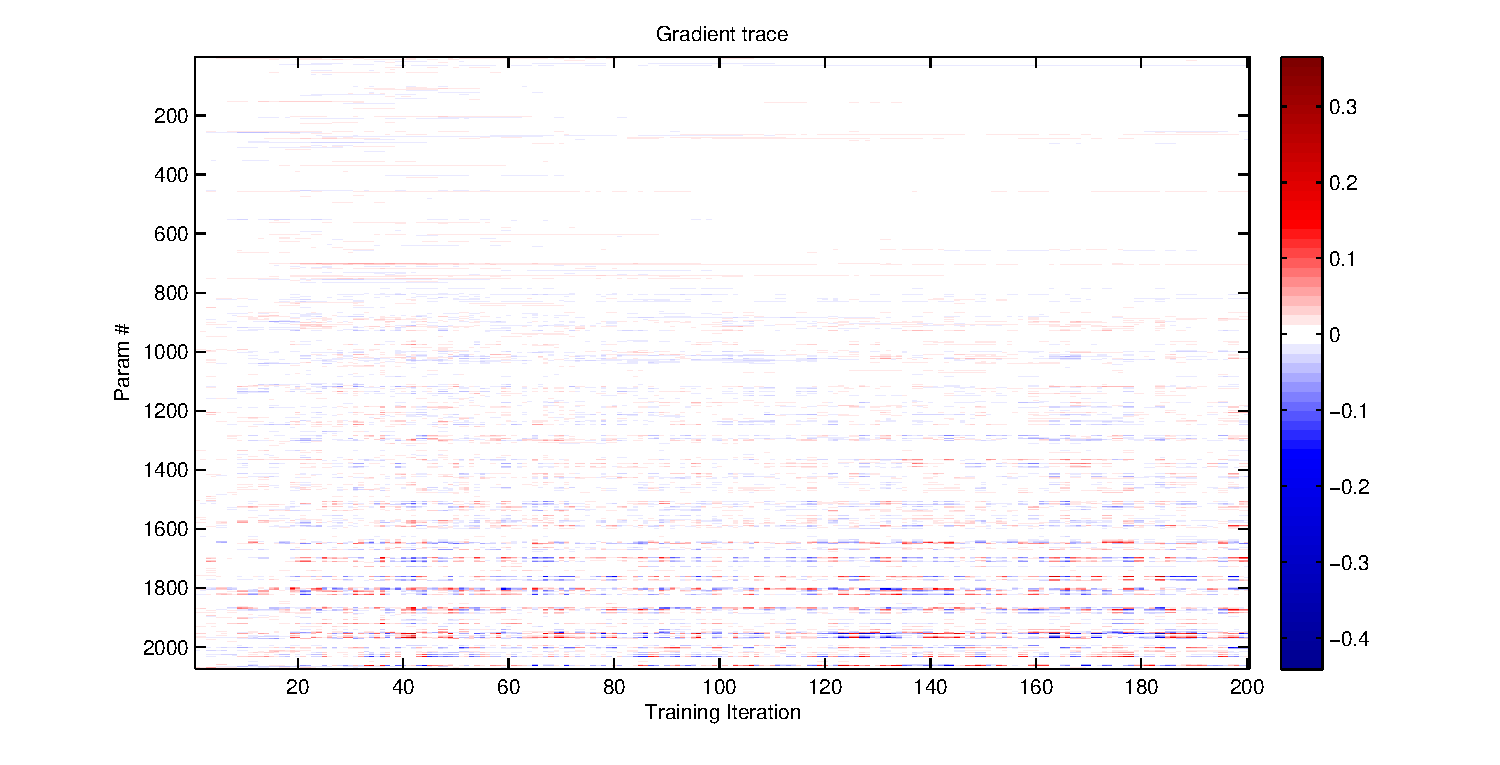
\includegraphics[width=0.9\linewidth]{ppt1}\\
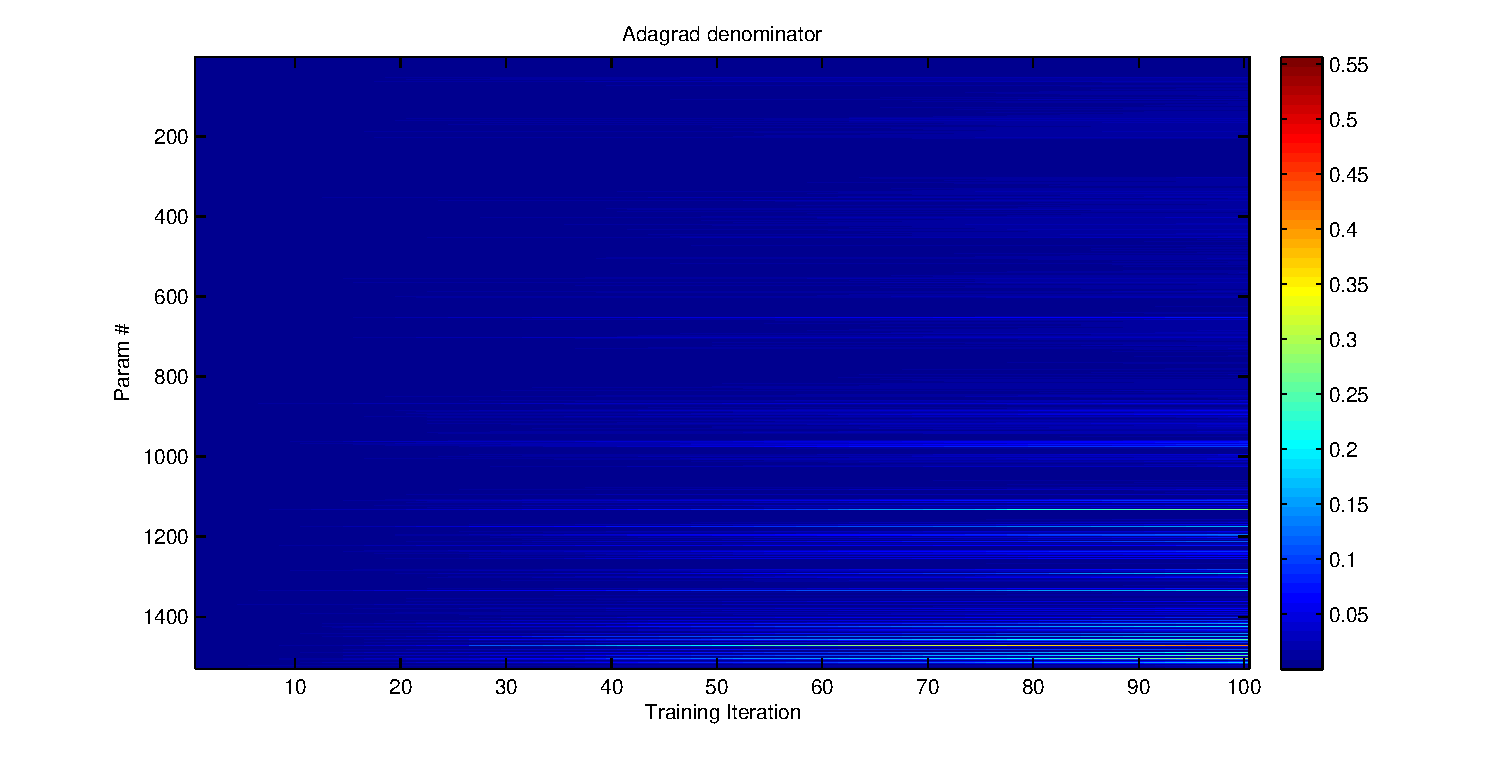
\includegraphics[width=0.9\linewidth]{ppt2}\\
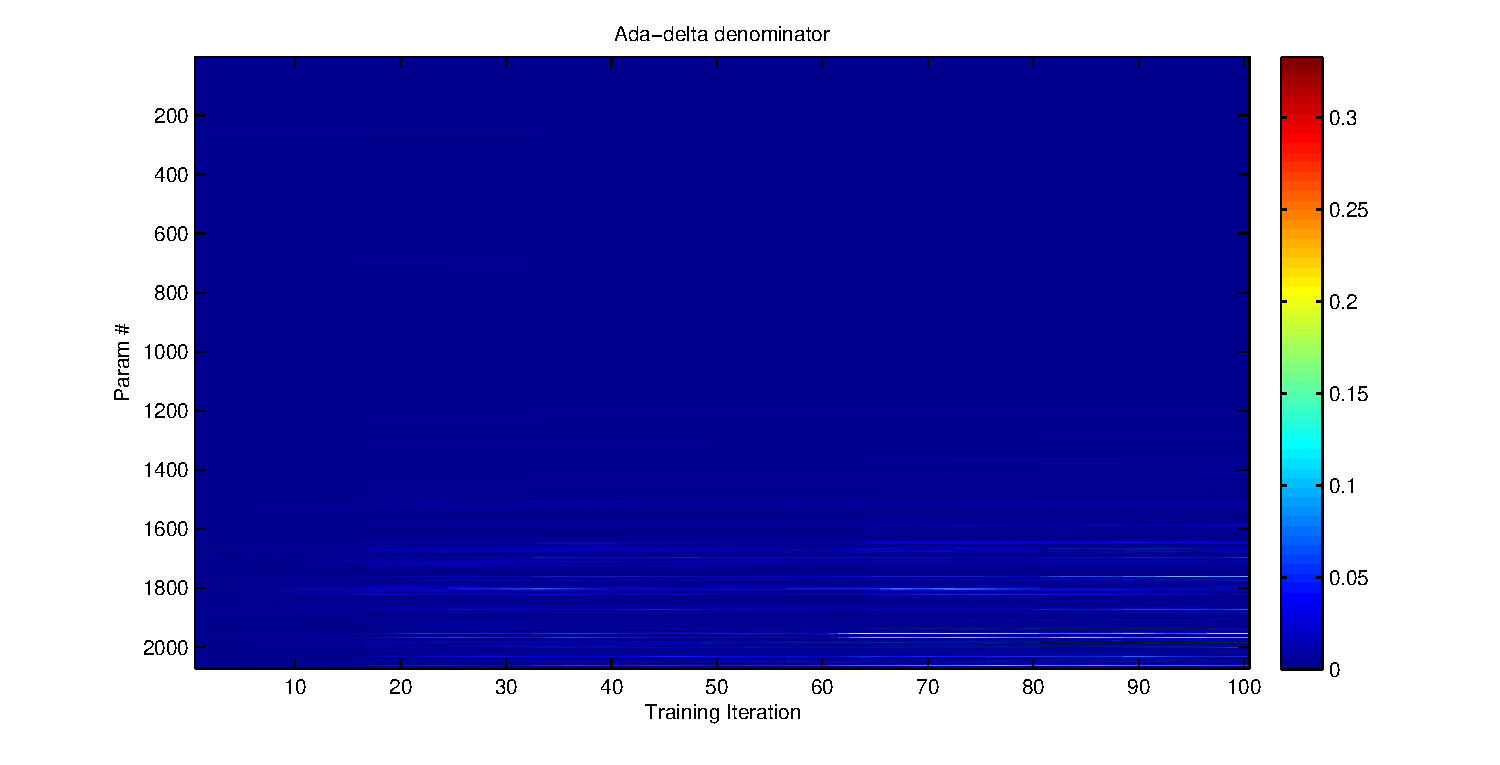
\includegraphics[width=0.9\linewidth]{ppt3}}
\caption{The gradient trace of training deep neural networks}\label{fig:grad_trace}
\end{figure}

These observations well support the intuitions for the algorithms we have experimented
with, and they seem to explain the fact that AdaGrad-based algorithms, when the step size 
problem is ameliorated, would outperform accelerated gradient methods by explicitly 
penalizing gradient components with high curvature and boosting the rest. From Figure 
\ref{fig:grad_trace} we can observe that the denominators for such adaptive gradient 
methods correctly capture the curvature properties in different gradient components, 
which would help to prevent the network parameters from oscillating and travel faster 
along the descent direction indicated by the low-curvature components.